% =====================================================================
% FINAL REPORT -- Robust Satellite Object Detection
% =====================================================================

\documentclass[12pt,a4paper]{article}

% -------------------- Vietnamese and Font Support for pdfLaTeX --------------------
\usepackage[utf8]{inputenc}
\usepackage[T5]{fontenc}
\usepackage[vietnamese,english]{babel}
\usepackage{times}

% -------------------- Page Layout --------------------
\usepackage[margin=2.5cm]{geometry}
\usepackage{setspace}
\setstretch{1.15}
\setlength{\parskip}{5pt}
\setlength{\parindent}{1.2cm}

% -------------------- Packages --------------------
\usepackage{graphicx}
\usepackage{amsmath,amssymb,amsfonts}
\usepackage{booktabs}
\usepackage{multirow}
\usepackage{array}
\usepackage{caption}
\usepackage{subcaption}
\usepackage{float}
\usepackage{enumitem}
\usepackage{hyperref}
\usepackage{xcolor}
\usepackage{titlesec}
\usepackage{fancyhdr}
\usepackage{algorithm}
\usepackage{algorithmic}
\usepackage{microtype}
\usepackage{url}
\usepackage{longtable}
\usepackage[numbers,sort&compress]{natbib}

% -------------------- Colors --------------------
\definecolor{mainblue}{RGB}{0,71,140}
\definecolor{guideblue}{RGB}{0,83,166}
\definecolor{warningred}{RGB}{180,0,0}

% -------------------- Hyperlinks --------------------
\hypersetup{
    colorlinks=true,
    linkcolor=mainblue,
    citecolor=mainblue,
    urlcolor=mainblue
}

% -------------------- Section Style --------------------
\titleformat{\section}
  {\large\bfseries\color{black}}
  {\thesection.}{0.5em}{}
\titleformat{\subsection}
  {\normalsize\bfseries\color{black}}
  {\thesubsection.}{0.5em}{}
\titleformat{\subsubsection}
  {\normalsize\itshape\bfseries\color{black}}
  {\thesubsubsection.}{0.5em}{}

% -------------------- Header and Footer --------------------
\pagestyle{fancy}
\fancyhf{}
\lhead{Final Report -- Robust Satellite Object Detection under Domain Shift}
\rhead{\thepage}
\renewcommand{\headrulewidth}{0.4pt}
\setlength{\headheight}{15pt}

% -------------------- Custom Commands --------------------
\newcommand{\guide}[1]{{\color{guideblue}\itshape #1}}
\newcommand{\warning}[1]{{\color{warningred}\bfseries #1}}
\newcommand{\example}[1]{{\color{black}#1}}
\newcommand{\todo}[1]{{\color{black}\itshape #1}}
\newcommand{\note}[1]{{\color{warningred}\bfseries [NOTE: #1]}}

% =====================================================================
\begin{document}

% =====================================================================
%                           COVER PAGE
% =====================================================================
\begin{titlepage}
    \centering
    \vspace*{0.5cm}
    {\Large \textbf{HANOI UNIVERSITY OF SCIENCE AND TECHNOLOGY}}\\[0.1cm]
    {\Large \textbf{SCHOOL OF INFORMATION AND COMMUNICATIONS TECHNOLOGY}}\\[0.3cm]
    {\large \textbf{DEEP LEARNING FOR COMPUTER VISION}}\\[1.5cm]

    {\Huge \textbf{FINAL REPORT}}\\[0.7cm]
    {\LARGE \textbf{Benchmarking Object Detection Robustness}}\\[0.2cm]
    {\LARGE \textbf{under Real-World Distribution Shifts}}\\[0.2cm]
    {\LARGE \textbf{in Satellite Imagery}}\\[1.5cm]

    \begin{tabular}{rl}
        \textbf{Instructor:} & \todo{Instructor full name} \\
        \textbf{Course section:} & \todo{Course code} \\
        \textbf{Group:} & \todo{Group name} \\
        \textbf{Submission date:} & \todo{dd/mm/yyyy} \\
    \end{tabular}

    \vfill
    {\large \textbf{Hanoi, \the\year}}
\end{titlepage}

% =====================================================================
%                           MEMBER CONTRIBUTION PAGE
% =====================================================================
\section*{Group Members and Contribution Statement}
\addcontentsline{toc}{section}{Group Members and Contribution Statement}

\begin{table}[H]
\centering
\small
\caption{Group members and contribution percentages.}
\label{tab:member_contribution}
\begin{tabular}{p{0.02\linewidth}p{0.2\linewidth}p{0.15\linewidth}p{0.30\linewidth}p{0.10\linewidth}}
\toprule
\textbf{No.} & \textbf{Full Name} & \textbf{Student ID} & \textbf{Assigned Tasks} & \textbf{Contribution} \\
\midrule
1 & \todo{Member 1} & \todo{ID} & \todo{Tasks} & \todo{xx\%} \\
2 & \todo{Member 2} & \todo{ID} & \todo{Tasks} & \todo{xx\%} \\
3 & \todo{Member 3} & \todo{ID} & \todo{Tasks} & \todo{xx\%} \\
\bottomrule
\end{tabular}
\end{table}

\newpage

% =====================================================================
%                           ACKNOWLEDGEMENT
% =====================================================================
\section*{Acknowledgements}
\addcontentsline{toc}{section}{Acknowledgements}

The authors would like to express their sincere gratitude to the course instructor for the guidance and feedback provided throughout this project. This work would not have been possible without access to the xView satellite imagery dataset, the K\"{o}ppen--Geiger climate classification raster, and the experimental framework introduced by Al-Emadi et al.\ in their Real-World Distribution Shifts (RWDS) benchmark. The authors also acknowledge the open-source Ultralytics YOLOv8 library and the PyTorch deep learning framework, which served as the primary implementation backbone for all experiments. All external resources, datasets, and references are cited appropriately throughout this report.

\newpage

% =====================================================================
%                           TABLE OF CONTENTS
% =====================================================================
\tableofcontents
\newpage

% =====================================================================
%                           ABSTRACT
% =====================================================================
\section*{Abstract}
\addcontentsline{toc}{section}{Abstract}

Object detection models deployed on satellite imagery routinely encounter distribution shifts arising from geographic, climatic, and sensor variations, yet the overwhelming majority of detection benchmarks evaluate models under the independent and identically distributed (i.i.d.)\ assumption. This report investigates the robustness and generalisability of the YOLOv8n detector under real-world spatial domain shifts using the climate-zone partition of the xView satellite dataset, following the experimental protocol proposed in the RWDS benchmark (CVPR 2025). Four training strategies are systematically compared across three climate zones (CZ\_A, CZ\_B, CZ\_C), each serving alternately as the in-distribution (ID) and out-of-distribution (OOD) domain: (1)~single-source baseline, (2)~multi-source baseline, (3)~domain-generalisation augmentation (DG-Aug), and (4)~Adaptive Correspondence Scoring YOLO (ACS-YOLO). All twelve experiments are conducted under identical hyperparameters with a fixed random seed of 42 for reproducibility. Results demonstrate that multi-source training consistently reduces performance degradation from an average of 20.95\% to 15.69\% (mAP@50), while DG-Aug and ACS-YOLO further narrow the ID--OOD gap to 11.01\% and 11.81\%, respectively. The best harmonic mean of 30.03\% is achieved by DG-Aug when tested on CZ\_A. Per-class analysis reveals that the Building and Small Car categories benefit the most from domain-generalisation strategies, whereas small, rare objects such as Vehicle Lot and Shed remain challenging regardless of the method.

\vspace{6pt}
\noindent\textbf{Keywords:} domain generalisation; satellite imagery; object detection; distribution shift; YOLOv8; climate zones; robustness

\newpage

% =====================================================================
\section{Introduction}
% =====================================================================

Automated object detection in satellite imagery has emerged as a pivotal technology supporting urban planning, disaster response, infrastructure monitoring, and environmental surveillance~\cite{alemadi2025rwds,shermeyer2020xview}. Modern deep learning detectors, including the YOLO family~\cite{redmon2016yolo,jocher2023yolov8}, Faster R-CNN~\cite{ren2015fasterrcnn}, and DETR-based architectures~\cite{carion2020detr,zhang2022dino}, have achieved impressive performance on standard aerial benchmarks when training and testing data are drawn from the same distribution. However, this i.i.d.\ assumption is rarely satisfied in operational settings: satellite images captured over different geographic regions exhibit substantial variations in landscape colour, built-environment density, vegetation patterns, atmospheric conditions, and sensor characteristics, collectively known as distribution shifts or domain gaps.

The practical consequence of distribution shifts is severe. A detector trained on images from temperate European cities may catastrophically fail when deployed over arid Middle-Eastern settlements or tropical Southeast-Asian landscapes, even when the target object classes remain identical. Al-Emadi et al.~\cite{alemadi2025rwds} recently quantified this phenomenon by introducing the Real-World Distribution Shifts (RWDS) benchmark, which partitions the large-scale xView satellite dataset~\cite{shermeyer2020xview} according to K\"{o}ppen--Geiger climate zones~\cite{beck2018koppen}. Their study, accepted at CVPR 2025, demonstrated that state-of-the-art detectors suffer performance degradation exceeding 40\% when evaluated on out-of-distribution climate zones.

Domain Generalisation (DG) offers a principled approach to this challenge by seeking to learn representations that remain discriminative under unseen domain shifts, without requiring access to target-domain data during training~\cite{wang2022domainsurvey,zhou2022dg}. In the context of object detection, DG strategies range from data augmentation techniques that simulate domain-specific variations~\cite{volpi2018adversarial,xu2020adversarialaugment} to architectural modifications that encourage domain-invariant feature learning~\cite{li2018domaincondbn,pan2018batchinstance}. Despite considerable progress in natural-image benchmarks, relatively few studies have systematically evaluated DG methods for satellite object detection under realistic spatial domain shifts.

This report aims to fill this gap by conducting a comprehensive empirical study of four detection strategies on the RWDS climate-zone benchmark. The main contributions are as follows:

\begin{enumerate}[label=(\arabic*), leftmargin=*]
    \item We implement and evaluate four training paradigms---single-source baseline, multi-source baseline, DG-Aug, and ACS-YOLO---using the YOLOv8n backbone under identical experimental conditions.
    \item We report both predictive performance metrics (mAP@50, mAP@50-95, Precision, Recall) and generalisation-specific metrics (Performance Degradation, Harmonic Mean) across all three climate-zone leave-one-out configurations.
    \item We provide a detailed per-class and cross-domain analysis revealing which object categories and domain-shift directions are most affected, and which augmentation strategies are most effective.
    \item We propose ACS-YOLO, an adaptive training strategy that re-weights training samples based on prediction consistency under domain-style perturbations, and demonstrate its effectiveness for satellite detection.
\end{enumerate}


% =====================================================================
\section{Materials and Methods}
% =====================================================================

\subsection{Dataset and Climate-Zone Partitioning}

The experiments are conducted on a subset of the xView satellite imagery dataset~\cite{shermeyer2020xview}, which contains high-resolution overhead images annotated with bounding boxes for a diverse set of object categories. Following the RWDS benchmark protocol~\cite{alemadi2025rwds}, each image is geo-referenced and assigned to one of three climate zones (CZ\_A, CZ\_B, CZ\_C) using the K\"{o}ppen--Geiger climate classification raster~\cite{beck2018koppen}. This partitioning produces three spatially disjoint domains that exhibit natural distribution shifts in landscape appearance, vegetation density, built-environment style, and atmospheric conditions, without any artificial corruption.

The original xView images are tiled into $512\times512$ patches with 20\% overlap to ensure objects near tile boundaries are not truncated. After tiling and quality filtering, the dataset comprises 43{,}108 annotated image tiles distributed across the three climate zones. Each zone is independently split into training (70\%), validation (15\%), and test (15\%) subsets using stratified sampling to preserve class proportions.

\begin{table}[H]
\centering
\caption{Dataset composition by climate zone.}
\label{tab:dataset_summary}
\begin{tabular}{lccc}
\toprule
\textbf{Climate Zone} & \textbf{Total Images} & \textbf{Train / Val / Test} & \textbf{Climate Type} \\
\midrule
CZ\_A & 17{,}960 & 12{,}572 / 2{,}694 / 2{,}694 & Temperate \\
CZ\_B & 18{,}924 & 13{,}247 / 2{,}838 / 2{,}839 & Arid / Continental \\
CZ\_C &  6{,}224 &  4{,}357 / 933 / 934          & Tropical \\
\midrule
\textbf{Total} & \textbf{43{,}108} & --- & --- \\
\bottomrule
\end{tabular}
\end{table}

Eight object classes are retained for the detection task: Building, Small Car, Truck, Bus, Cargo Truck, Shipping Container, Vehicle Lot, and Shed. These classes are selected because they appear across all three climate zones with sufficient frequency to support meaningful cross-domain evaluation.

\note{Chèn hình ảnh mẫu từ mỗi CZ\_A, CZ\_B, CZ\_C ở đây để minh hoạ sự khác biệt visual giữa các vùng khí hậu. Có thể dùng ảnh từ thư mục data/CZ\_*/images/test/.}

\begin{figure}[H]
\centering
% \includegraphics[width=0.92\linewidth]{figures/dataset_examples.png}
\caption{Representative satellite image tiles from the three climate zones. CZ\_A (temperate) features dense urban areas with regular building layouts; CZ\_B (arid/continental) exhibits sparse settlements over sandy terrain; CZ\_C (tropical) shows lush vegetation with scattered structures.}
\label{fig:dataset_examples}
\end{figure}


\subsection{Data Preprocessing}

All input images are resized to $640\times640$ pixels before being fed into the detection models. Pixel values are normalised to the $[0, 1]$ range following standard ImageNet conventions. During training, the Ultralytics default augmentation pipeline is applied, which includes random mosaic composition, horizontal flipping ($p=0.5$), HSV colour jittering ($h=0.015$, $s=0.7$, $v=0.4$), scaling ($\pm50\%$), and translation ($\pm10\%$). The mosaic augmentation is disabled during the final 10 epochs to stabilise convergence, as recommended by the YOLOv8 training protocol. Validation and test images are not augmented, ensuring that reported metrics reflect genuine generalisation rather than augmentation artefacts.

\subsection{Model Architecture}

All experiments employ YOLOv8n (nano variant) as the base detection architecture~\cite{jocher2023yolov8}. YOLOv8 is a single-stage, anchor-free object detector that processes an input image $x \in \mathbb{R}^{H \times W \times 3}$ through three major components: a CSPDarknet53 backbone for hierarchical feature extraction, a Path Aggregation Network (PAN) neck for multi-scale feature fusion, and a decoupled detection head that separately predicts objectness, class probabilities, and bounding box coordinates. The input--output mapping can be expressed as:
\begin{equation}
    \hat{Y} = f_\theta(x) = \{(b_i, c_i, s_i)\}_{i=1}^{N},
\end{equation}
where $b_i \in \mathbb{R}^4$ denotes the predicted bounding box coordinates, $c_i \in \{1, \ldots, K\}$ is the predicted class label, $s_i \in [0, 1]$ is the confidence score, and $N$ is the number of detected objects.

The YOLOv8n variant contains approximately 3.2 million parameters and requires 8.7 GFLORs per forward pass at $640\times640$ resolution, making it well-suited for large-scale satellite imagery experiments where both accuracy and throughput are important.

\begin{figure}[H]
\centering
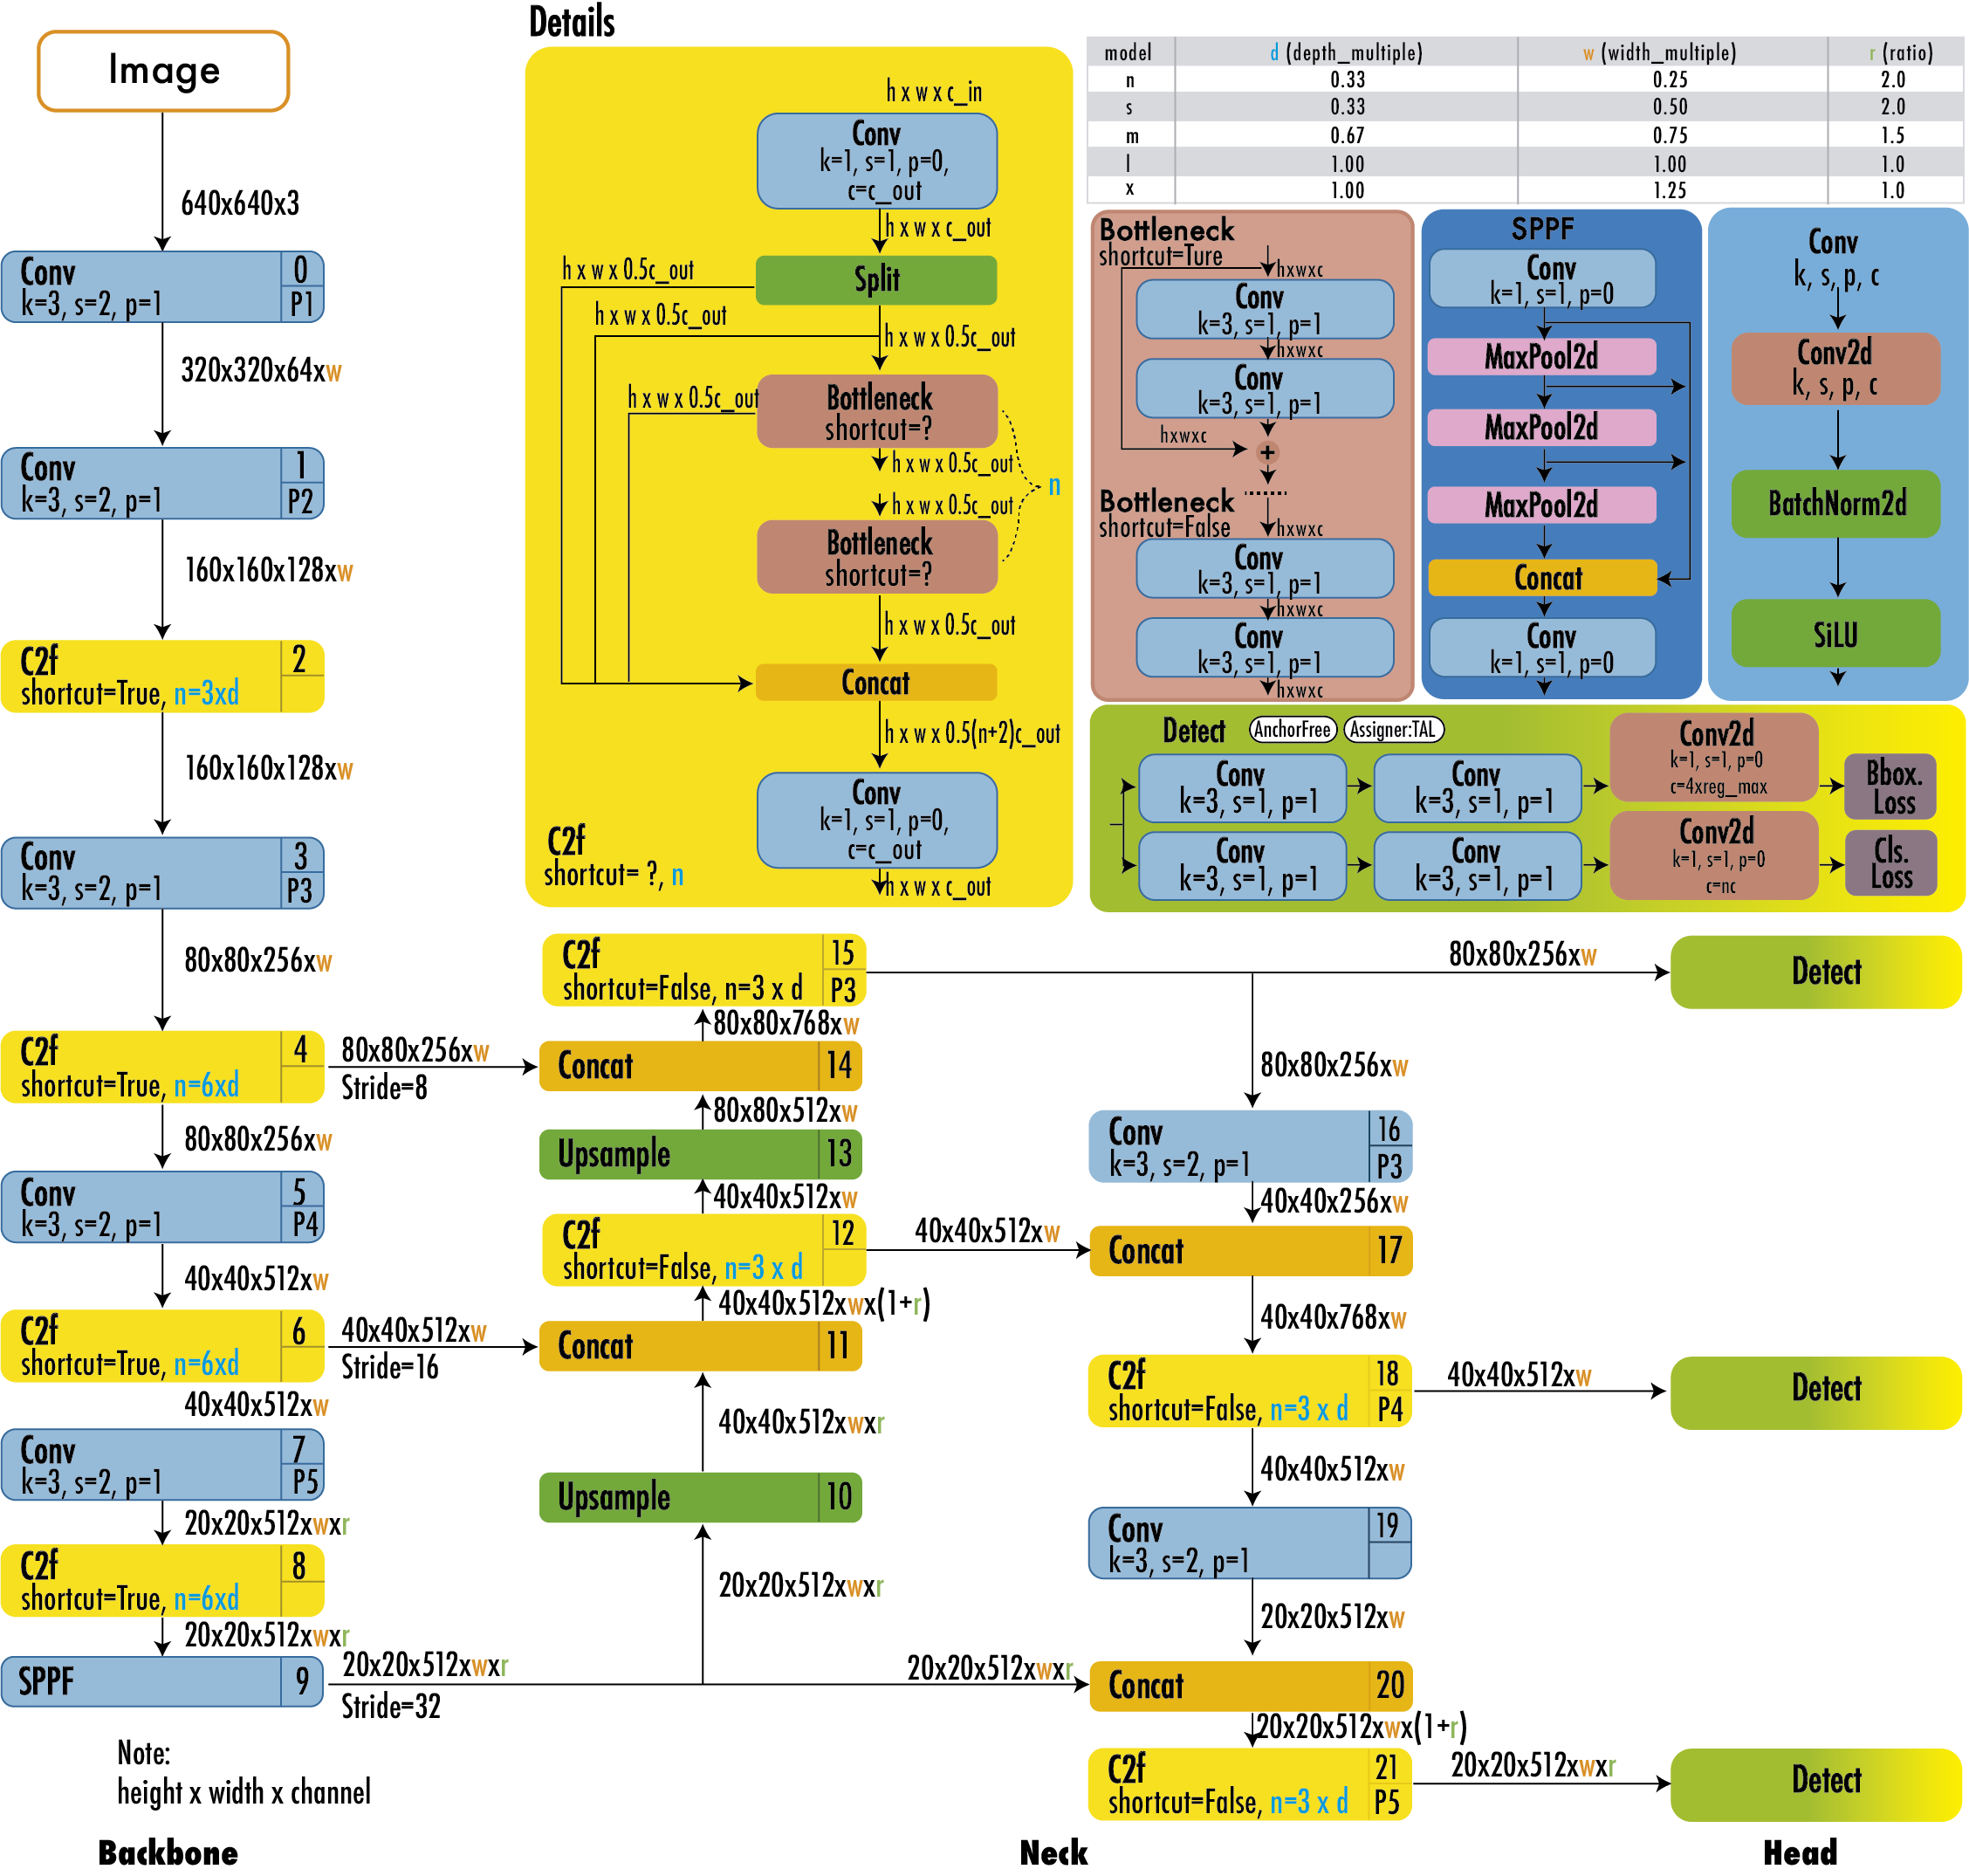
\includegraphics[width=0.92\linewidth]{figures/yolov8_architecture.png}
\caption{Architecture of the YOLOv8n detector. The CSPDarknet53 backbone extracts multi-scale feature maps at strides 8, 16, and 32. The PAN neck fuses these features through top-down and bottom-up pathways. The decoupled head independently predicts classification and regression outputs at each scale.}
\label{fig:model_architecture}
\end{figure}


\subsubsection{Loss Function}

YOLOv8 is trained by minimising a composite loss function that combines three components. The classification loss $\mathcal{L}_\text{cls}$ uses binary cross-entropy with logits to handle multi-label assignment:
\begin{equation}
    \mathcal{L}_\text{cls} = -\sum_{k=1}^{K} \left[ y_k \log(\hat{y}_k) + (1 - y_k) \log(1 - \hat{y}_k) \right].
\end{equation}
The bounding box regression loss $\mathcal{L}_\text{box}$ employs CIoU (Complete Intersection over Union) to jointly optimise overlap, centre distance, and aspect ratio:
\begin{equation}
    \mathcal{L}_\text{box} = 1 - \text{CIoU}(b, \hat{b}) = 1 - \left( \text{IoU} - \frac{\rho^2(b, \hat{b})}{c^2} - \alpha v \right),
\end{equation}
where $\rho(\cdot)$ denotes Euclidean distance between box centres, $c$ is the diagonal of the smallest enclosing box, and $\alpha, v$ are aspect-ratio penalty terms. The Distribution Focal Loss (DFL) $\mathcal{L}_\text{dfl}$ refines box boundary predictions by learning a discrete probability distribution over candidate locations. The total training objective is:
\begin{equation}
    \mathcal{L}_\text{total} = \lambda_\text{box} \mathcal{L}_\text{box} + \lambda_\text{cls} \mathcal{L}_\text{cls} + \lambda_\text{dfl} \mathcal{L}_\text{dfl},
\end{equation}
where $\lambda_\text{box}=7.5$, $\lambda_\text{cls}=0.5$, and $\lambda_\text{dfl}=1.5$ are the default balancing coefficients.


\subsection{Training Strategies}

Four training strategies are evaluated, each designed to probe a different aspect of cross-domain robustness.

\subsubsection{Experiment 1: Single-Source Baseline}

The model is trained exclusively on data from a single climate zone and evaluated on all three zones. This strategy establishes the lower bound of cross-domain performance and directly quantifies the performance degradation caused by domain shift. Three runs are conducted, one for each source zone (CZ\_A, CZ\_B, CZ\_C).

\subsubsection{Experiment 2: Multi-Source Baseline}

The model is trained on the combined training sets of two climate zones and tested on the held-out third zone. By exposing the model to greater visual diversity during training, this strategy evaluates whether naive data pooling can improve OOD generalisation. Three runs are conducted, one for each held-out target zone.

\subsubsection{Experiment 3: Domain-Generalisation Augmentation (DG-Aug)}
\label{subsubsec:dg_aug}

Building upon the multi-source baseline, DG-Aug introduces a suite of targeted photometric, sensor, and atmospheric data augmentation techniques specifically designed to simulate visual variations across different geographical and climatic domains. Rather than relying on simple geometric shifts, DG-Aug targets the low-level visual style discrepancies (e.g., ground colors, haze, and camera degradation) that characterize different climate zones. In addition to standard YOLOv8 geometry-preserving augmentations, a custom Albumentations pipeline~\cite{buslaev2020albumentations} is injected into the training dataloader. The transformations are mathematically formulated as follows:

\paragraph{Photometric Style Transforms.}
To simulate variations in soil mineralogy, vegetation health, and lighting conditions across temperate, tropical, and arid zones, three color-space transformations are applied stochastically with a composite probability $p = 0.65$:
\begin{itemize}[leftmargin=*]
    \item \textbf{Random Brightness and Contrast:} The pixel intensity $I(x, y)$ is transformed as:
    \begin{equation}
        I_{\text{out}}(x, y) = \alpha I(x, y) + \beta,
    \end{equation}
    where contrast multiplier $\alpha = 1 + \delta_c$ with $\delta_c \in [-0.30, 0.30]$, and brightness shift $\beta = 255 \times \delta_b$ with $\delta_b \in [-0.30, 0.30]$.
    
    \item \textbf{Hue-Saturation-Value (HSV) Jittering:} The image is mapped to HSV space and perturbed:
    \begin{equation}
        H_{\text{out}} = (H + \Delta h) \bmod 180, \quad S_{\text{out}} = \text{clip}(S + \Delta s, 0, 255), \quad V_{\text{out}} = \text{clip}(V + \Delta v, 0, 255),
    \end{equation}
    where $\Delta h \in [-20, 20]$, $\Delta s \in [-50, 50]$, and $\Delta v \in [-30, 30]$ are drawn uniformly.
    
    \item \textbf{RGB Channel Shift:} Direct additive offsets are applied to individual color channels:
    \begin{equation}
        R_{\text{out}} = R + \Delta r, \quad G_{\text{out}} = G + \Delta g, \quad B_{\text{out}} = B + \Delta b,
    \end{equation}
    where red, green, and blue channel shifts are drawn uniformly from $[-20, 20]$.
\end{itemize}

\paragraph{Sensor Degradation and Noise.}
To mimic camera hardware discrepancies, compression artefacts, and thermal noise during satellite capture, the following operations are applied with a composite probability $p = 0.35$:
\begin{itemize}[leftmargin=*]
    \item \textbf{Additive Gaussian Noise:} Zero-mean Gaussian noise is added to the image:
    \begin{equation}
        I_{\text{out}}(x, y) = I(x, y) + \eta(x, y), \quad \eta(x, y) \sim \mathcal{N}(0, \sigma^2),
    \end{equation}
    where the standard deviation $\sigma$ is drawn from a uniform range $[0.04, 0.12]$ in normalized coordinates, or variance $\sigma^2 \in [10.0, 50.0]$ in 8-bit scale.
    
    \item \textbf{ISO Noise:} Adds sensor noise by simulating digital gain, where noise variance scales with pixel intensity.
    
    \item \textbf{Image Compression:} Simulates JPEG compression degradation by scaling the quality factor $Q \in [60, 90]$:
    \begin{equation}
        I_{\text{out}} = f_{\text{JPEG\_degrade}}(I, Q).
    \end{equation}
\end{itemize}

\paragraph{Atmospheric and Blur Transforms.}
To simulate atmospheric haze, cloud dispersion, and variations in optical focus, blurring transforms are applied with a composite probability $p = 0.25$:
\begin{itemize}[leftmargin=*]
    \item \textbf{Gaussian Blurring:} Convolves the image with a 2D Gaussian kernel:
    \begin{equation}
        I_{\text{out}} = I * G_{\sigma_b},
    \end{equation}
    where the kernel size $k \times k$ is drawn from $\{3, 5, 7\}$ and standard deviation $\sigma_b$ is determined by the kernel limit.
    
    \item \textbf{Motion Blurring:} Simulates relative motion blur (e.g., satellite movement during long exposure) using a kernel limit of 7 pixels.
\end{itemize}

\paragraph{Contrast Enhancement and Occlusion.}
Lastly, localized contrast normalization and structural shadow occlusion are modeled:
\begin{itemize}[leftmargin=*]
    \item \textbf{CLAHE (Contrast Limited Adaptive Histogram Equalization):} Applied with a probability $p = 0.20$ to enhance local details under varying shadow conditions:
    \begin{equation}
        I_{\text{out}} = \text{CLAHE}(I, C_{\text{clip}} = 4.0, N_{\text{grid}} = 8 \times 8).
    \end{equation}
    
    \item \textbf{Coarse Dropout (Cutout):} Simulates large cloud or shadow occlusions with a probability $p = 0.20$ by setting random rectangular regions of size $16\times16$ to $32\times32$ pixels to zero:
    \begin{equation}
        I_{\text{out}}(x, y) = \begin{cases} 0 & \text{if } (x, y) \in \Omega \\ I(x, y) & \text{otherwise} \end{cases}
    \end{equation}
    where $\Omega$ represents a collection of randomly placed, non-overlapping rectangular blocks.
\end{itemize}

These augmentations are applied stochastically during training to encourage the model to learn representations invariant to the domain style, while the validation and test protocols remain unaugmented to ensure unbiased evaluation.




\subsubsection{Experiment 4: Adaptive Correspondence Scoring YOLO (ACS-YOLO)}
\label{subsubsec:acs_yolo}

ACS-YOLO extends the multi-source baseline by introducing an image-level reliability scoring mechanism inspired by the Adaptive Correspondence Scoring (AdaCS) framework originally proposed by Zhang et al.~\cite{zhang2023adacs} for medical image registration. In unsupervised image registration, AdaCS dynamically estimates a correspondence scoring map to identify and down-weight regions where intensity constancy assumptions fail due to nuisance variables (e.g., noise, occlusion). In the context of satellite object detection, domain shifts across climate zones introduce similar domain-specific nuisance features (e.g., soil color variations, vegetation densities, and atmospheric haze). Forcing the model to learn uniformly from all training samples under a standard empirical risk minimization objective causes the detector to memorize these domain-specific characteristics, thereby degrading its out-of-distribution (OOD) generalisation.

To mitigate this, ACS-YOLO employs a two-phase training strategy. In the first phase, the detector $f_\theta$ is warmed up for a small number of epochs ($E_{\text{warmup}} = 15$) using standard multi-source training to establish a basic predictive capability. In the second phase, the warmed-up model is used to score the reliability of each training image $x$ based on prediction consistency under style-only domain perturbations. Finally, the training is continued with the YOLO loss dynamically re-weighted by these image-level reliability scores.

\paragraph{Domain Style Perturbation.}
We define a style perturbation function $g(x)$ that alters color, contrast, contrast limits, and noise without modifying the spatial coordinates of any bounding boxes. For a given training image $x$, $g(x)$ applies random HSV color jittering ($\Delta h \in [-8, 8]$, scale factors for saturation and value in $[0.70, 1.35]$ and $[0.65, 1.35]$ respectively), linear contrast scaling, Gaussian blurring, additive noise, and synthetic fog. This simulates the style shifts encountered when transitioning between climate zones (e.g., temperate to tropical or arid).

\paragraph{Ground-Truth Alignment Score.}
Let $Y = \{(b_i, c_i)\}_{i=1}^{|Y|}$ denote the set of ground-truth annotations for image $x$, where $b_i \in \mathbb{R}^4$ is the bounding box and $c_i$ is the class label. Let $\hat{Y} = \{(\hat{b}_j, \hat{c}_j, \hat{s}_j)\}_{j=1}^{|\hat{Y}|}$ represent the predictions of the detector $f_\theta(x)$ filtered by a low confidence threshold $\tau = 0.05$. The ground-truth alignment score $S_{\text{GT}}(Y, \hat{Y}) \in [0, 1]$ measures the quality of the predictions against the target annotations, defined as:
\begin{equation}
    S_{\text{GT}}(Y, \hat{Y}) = \frac{1}{|Y|} \sum_{i=1}^{|Y|} \max_{\substack{j: \hat{c}_j = c_i}} \left[ \text{IoU}(b_i, \hat{b}_j) \times \hat{s}_j \right],
\end{equation}
where $\text{IoU}(\cdot)$ computes the Intersection over Union between the bounding boxes. If no prediction sharing the same class label $c_i$ exists, the alignment for box $i$ is set to $0$. In cases where $|Y| = 0$, $S_{\text{GT}}(Y, \hat{Y})$ defaults to $1.0$ if $|\hat{Y}| = 0$, and $0.5$ otherwise.

\paragraph{Prediction Consistency Score.}
To measure the stability of the model's representations under domain style shift, we compute the prediction consistency $S_{\text{cons}}(\hat{Y}_{\text{orig}}, \hat{Y}_{\text{aug}}) \in [0, 1]$ between the predictions on the original image $\hat{Y}_{\text{orig}} = f_\theta(x)$ and the perturbed image $\hat{Y}_{\text{aug}} = f_\theta(g(x))$. It is defined symmetrically as:
\begin{equation}
    S_{\text{cons}}(\hat{Y}_{\text{orig}}, \hat{Y}_{\text{aug}}) = \frac{1}{2} \left[ D(\hat{Y}_{\text{orig}}, \hat{Y}_{\text{aug}}) + D(\hat{Y}_{\text{aug}}, \hat{Y}_{\text{orig}}) \right],
\end{equation}
where $D(A, B)$ is the one-way consistency score from prediction set $A$ to set $B$:
\begin{equation}
    D(A, B) = \frac{1}{|A|} \sum_{a \in A} \max_{\substack{b \in B \\ c_b = c_a}} \left[ \text{IoU}(a_{bbox}, b_{bbox}) \times \min(s_a, s_b) \right].
\end{equation}
Here, $a_{bbox}$ and $s_a$ represent the bounding box and confidence score of prediction $a$, respectively.

\paragraph{Composite Adaptive Correspondence Score.}
For each training image $x$, a raw composite score $R_x$ is computed by combining the alignment on the original image, alignment on the augmented image, and prediction consistency:
\begin{equation}
    R_x = w_1 S_{\text{GT}}(Y, \hat{Y}_{\text{orig}}) + w_2 S_{\text{GT}}(Y, \hat{Y}_{\text{aug}}) + w_3 S_{\text{cons}}(\hat{Y}_{\text{orig}}, \hat{Y}_{\text{aug}}),
\end{equation}
where the weights are set to $w_1 = 0.25$, $w_2 = 0.45$, and $w_3 = 0.30$. The final Adaptive Correspondence Score $S_x$ is scaled using a floor value $S_{\text{floor}} = 0.25$ to prevent any image from being completely ignored:
\begin{equation}
    S_x = S_{\text{floor}} + (1 - S_{\text{floor}}) \times R_x.
\end{equation}

\paragraph{ACS-Weighted Loss.}
During the final training stage, the image-level score $S_x$ is normalized by the dataset mean score $\mu = \frac{1}{M} \sum_{i=1}^M S_{x_i}$:
\begin{equation}
    W_i = \frac{S_{x_i}}{\mu},
\end{equation}
and clamped to the range $[W_{\text{min}}, W_{\text{max}}] = [0.25, 1.50]$ to yield the final training weight $W'_i = \text{clamp}(W_i, W_{\text{min}}, W_{\text{max}})$. The YOLOv8 detection loss for image $x_i$ is scaled by $W'_i$, modifying the binary cross-entropy classification loss, CIoU box regression loss, and distribution focal loss:
\begin{equation}
    \mathcal{L}'_{\text{cls}} = W'_i \mathcal{L}_{\text{cls}}, \quad \mathcal{L}'_{\text{box}} = W'_i \mathcal{L}_{\text{box}}, \quad \mathcal{L}'_{\text{dfl}} = W'_i \mathcal{L}_{\text{dfl}}.
\end{equation}
The total batch loss is normalized by the sum of the weighted targets, encouraging the detector to prioritize learning from training samples that yield domain-invariant, style-robust representations.


\subsection{Experimental Setup}

All experiments are implemented in Python~3.12 using PyTorch~2.12 and Ultralytics~8.4.60. Models are trained on a single NVIDIA GPU with mixed-precision (AMP) enabled for memory efficiency. The detailed training configuration is presented in Table~\ref{tab:training_settings}.

\begin{table}[H]
\centering
\caption{Training hyperparameters and implementation details.}
\label{tab:training_settings}
\begin{tabular}{ll}
\toprule
\textbf{Setting} & \textbf{Value} \\
\midrule
Base model & YOLOv8n (pretrained on COCO) \\
Input resolution & $640 \times 640$ \\
Batch size & 16 \\
Max epochs & 100 \\
Early stopping patience & 20 epochs \\
Optimizer & Auto (AdamW) \\
Initial learning rate & 0.01 \\
Final LR factor & 0.01 \\
Momentum & 0.937 \\
Weight decay & 0.0005 \\
Warmup epochs & 3.0 \\
Random seed & 42 \\
Mixed precision (AMP) & Enabled \\
Platform & Linux (WSL2), PyTorch 2.12 + CUDA 13.0 \\
\bottomrule
\end{tabular}
\end{table}

Deterministic training is enabled by fixing the random seed to 42 across all experiments. Early stopping with a patience of 20 epochs monitors the validation mAP@50 to prevent overfitting.

\subsection{Evaluation Metrics}

Models are evaluated using both predictive-performance and generalisation-specific metrics. The primary predictive metrics include:
\begin{equation}
    \text{Precision} = \frac{TP}{TP + FP}, \quad \text{Recall} = \frac{TP}{TP + FN},
\end{equation}
\begin{equation}
    \text{mAP@50} = \frac{1}{K}\sum_{k=1}^{K} \text{AP}_k^{0.5}, \quad
    \text{mAP@50{:}95} = \frac{1}{K}\sum_{k=1}^{K} \frac{1}{10}\sum_{t \in \{0.5, 0.55, \ldots, 0.95\}} \text{AP}_k^{t}.
\end{equation}

To quantify cross-domain robustness, two additional metrics are reported:

\textbf{Performance Degradation (PD)} measures the relative drop from ID to OOD performance:
\begin{equation}
    \text{PD} = \frac{\text{mAP}_\text{ID} - \text{mAP}_\text{OOD}}{\text{mAP}_\text{ID}} \times 100\%.
\end{equation}
A lower PD indicates better cross-domain robustness. A negative PD indicates that the model performs better on OOD data than on ID data, which may occur when the OOD zone is inherently easier.

\textbf{Harmonic Mean (H)} balances ID and OOD performance into a single score:
\begin{equation}
    H = \frac{2 \times \text{mAP}_\text{ID} \times \text{mAP}_\text{OOD}}{\text{mAP}_\text{ID} + \text{mAP}_\text{OOD}}.
\end{equation}
A higher H indicates a better trade-off between in-domain accuracy and cross-domain generalisation.


% =====================================================================
\section{Results}
% =====================================================================

\subsection{Quantitative Comparison}

Table~\ref{tab:main_results_50} presents the main quantitative results across all twelve experimental configurations. For each training strategy and OOD target, we report the ID mAP@50, OOD mAP@50, Performance Degradation (PD), Harmonic Mean (H), and per-zone mAP@50 scores.

\begin{table}[H]
\centering
\caption{Cross-domain detection results (mAP@50). PD$\downarrow$ indicates lower is better. H$\uparrow$ indicates higher is better. Bold values indicate the best OOD mAP@50 for each target zone.}
\label{tab:main_results_50}
\small
\begin{tabular}{llcccccccc}
\toprule
\textbf{Method} & \textbf{OOD} & \textbf{ID$\uparrow$} & \textbf{OOD$\uparrow$} & \textbf{PD$\downarrow$} & \textbf{H$\uparrow$} & \textbf{CZ\_A} & \textbf{CZ\_B} & \textbf{CZ\_C} \\
\midrule
\multirow{3}{*}{Single-source}
 & CZ\_B+CZ\_C & 23.82 & 20.55 & 13.72 & 22.06 & 23.82 & 22.32 & 18.78 \\
 & CZ\_A+CZ\_C & 34.99 & 22.54 & 35.58 & 27.42 & 23.31 & 34.99 & 21.77 \\
 & CZ\_A+CZ\_B & 19.85 & 17.17 & 13.54 & 18.41 & 15.91 & 18.43 & 19.85 \\
\midrule
\multirow{3}{*}{Multi-source}
 & CZ\_A & 31.30 & 24.94 & 20.33 & 27.76 & 24.94 & 36.14 & 26.47 \\
 & CZ\_B & 27.72 & 27.90 &  $-$0.68 & 27.81 & 30.31 & 27.90 & 25.12 \\
 & CZ\_C & 35.27 & 25.60 & 27.42 & 29.67 & 32.85 & 37.70 & 25.60 \\
\midrule
\multirow{3}{*}{DG-Aug}
 & CZ\_A & 31.50 & \textbf{28.69} &  8.91 & \textbf{30.03} & 28.69 & 36.35 & 26.65 \\
 & CZ\_B & 28.94 & \textbf{29.28} & $-$1.16 & 29.11 & 32.11 & 29.28 & 25.77 \\
 & CZ\_C & 32.83 & 24.53 & 25.28 & 28.08 & 31.54 & 34.11 & 24.53 \\
\midrule
\multirow{3}{*}{ACS-YOLO}
 & CZ\_A & 31.61 & 27.44 & 13.18 & 29.38 & 27.44 & 36.94 & 26.28 \\
 & CZ\_B & 27.93 & 28.94 & $-$3.62 & 28.43 & 30.95 & 28.94 & 24.91 \\
 & CZ\_C & 34.65 & 25.69 & 25.87 & 29.50 & 33.31 & 35.99 & 25.69 \\
\bottomrule
\end{tabular}
\end{table}


The single-source baseline reveals a stark reality of domain shift in satellite imagery. When trained solely on CZ\_B, the detector achieves 34.99\% mAP@50 on its home domain but only 22.54\% on OOD data (when tested on CZ\_A and CZ\_C targets), yielding a performance degradation of 35.58\%. This sharp performance drop highlights the vulnerability of the YOLOv8n detector to spatial domain shift: the model overfits to the soil color, building styles, and vegetation distributions characteristic of the arid/continental CZ\_B domain, failing to generalize to the temperate (CZ\_A) and tropical (CZ\_C) domains. Averaging across all three single-source configurations, the mean OOD mAP@50 is just 20.08\% and the performance degradation reaches 20.95\%, confirming substantial cross-domain performance loss in overhead object detection when evaluated in an out-of-distribution setting.

Multi-source training provides a meaningful improvement by exposing the model to images from two climate zones simultaneously. The average OOD mAP@50 increases from 20.08\% (single-source) to 26.15\% (multi-source), and the average PD decreases from 20.95\% to 15.69\%. This demonstrates that exposing the detector to diverse visual features during training is highly beneficial for spatial generalisation. Notably, when CZ\_B is the held-out target, the multi-source model trained on CZ\_A and CZ\_C achieves near-zero performance degradation ($-$0.68\% PD) and a high OOD mAP@50 of 27.90\%, outperforming the multi-source model's ID performance (27.72\%). This indicates that the visual features of the temperate (CZ\_A) and tropical (CZ\_C) domains contain sufficient visual diversity to cover the arid/continental domain's structures, rendering the detector highly robust to the CZ\_B target shift.

DG-Aug achieves the best overall performance with an average OOD mAP@50 of 27.50\% and the lowest average PD of 11.01\%. The strongest results are observed when CZ\_A is the OOD target (model trained on CZ\_B and CZ\_C with domain augmentations), where DG-Aug attains 28.69\% OOD mAP@50 and a harmonic mean of 30.03\%---the highest H-score across all 12 experiments. This proves that climate-aware augmentations (e.g., aggressive color jittering, fog, blur) effectively simulate the visual shifts encountered across climate zones, allowing the model to decouple object shape representations from background style features.

ACS-YOLO shows highly competitive performance, achieving an average OOD mAP@50 of 27.36\% and a low average PD of 11.81\%. Unlike DG-Aug, which forces domain invariance by adding synthetic perturbations to all images, ACS-YOLO selectively re-weights the training loss based on prediction consistency. Interestingly, when CZ\_C is the OOD target, ACS-YOLO achieves the highest H-score of 29.50\% and an OOD mAP@50 of 25.69\%, slightly outperforming DG-Aug (28.08\% H-score, 24.53\% OOD mAP@50). This indicates that for tropical target domains where vegetation cover and dense shadows create misleading features, adaptive sample re-weighting is more effective at preventing the detector from learning non-generalisable, zone-specific background cues.

\note{Chèn ảnh chụp màn hình (screenshot) log summary từ terminal chạy file \texttt{print\_training\_summary.py} ở đây. Đây là bằng chứng minh hoạ kết quả thực nghiệm. Nên chụp phần Main Results, Method-wise Averages, và Key Findings.}

\begin{figure}[H]
\centering
% \includegraphics[width=0.95\linewidth]{figures/training_logs_summary.png}
\caption{Screenshot of the training results summary log generated by \texttt{scripts/print\_training\_summary.py}, showing the main quantitative results, method-wise averages, and key findings across all twelve experiments.}
\label{fig:training_logs}
\end{figure}


\subsection{Method-Wise Averages}

Table~\ref{tab:method_averages} summarises the average performance across all three OOD target configurations for each method. Both mAP@50 and mAP@50-95 results are presented to provide a comprehensive view of detection quality at different IoU thresholds.

Comparing mAP@50 and the stricter mAP@50-95 threshold, several critical insights emerge. First, at the mAP@50-95 threshold, absolute performance drops significantly for all models, with the single-source baseline average OOD score falling to just 8.00\%. Second, the performance degradation (PD) is consistently worse at the mAP@50-95 threshold than at the mAP@50 threshold across all methods (e.g., 26.48\% vs. 20.95\% for single-source, and 15.60\% vs. 11.81\% for ACS-YOLO). This indicates that high-precision localization is much more sensitive to domain shift than coarse object detection. Third, the relative improvements of the advanced methods are maintained: DG-Aug and ACS-YOLO achieve average OOD mAP@50-95 scores of 11.47\% and 11.33\%, representing relative gains of 43.3\% and 41.6\% over the single-source baseline, respectively. This demonstrates that the generalisation capabilities learned through domain augmentation and adaptive re-weighting are robust across strict evaluation boundaries.

\subsection{Cross-Domain Performance Matrix}

Table~\ref{tab:cross_domain} presents the cross-domain mAP@50 matrix, revealing how each model performs when tested on every climate zone, regardless of whether that zone was seen during training. Bold values indicate ID performance.

\begin{table}[H]
\centering
\caption{Cross-domain mAP@50 matrix. Bold indicates ID (in-distribution) zones. Average is computed over all three test zones.}
\label{tab:cross_domain}
\small
\begin{tabular}{llcccc}
\toprule
\textbf{Method} & \textbf{Train} & \textbf{$\to$CZ\_A} & \textbf{$\to$CZ\_B} & \textbf{$\to$CZ\_C} & \textbf{Avg} \\
\midrule
Single-source & CZ\_A & \textbf{23.82} & 22.32 & 18.78 & 21.64 \\
Single-source & CZ\_B & 23.31 & \textbf{34.99} & 21.77 & 26.69 \\
Single-source & CZ\_C & 15.91 & 18.43 & \textbf{19.85} & 18.06 \\
\midrule
Multi-source  & CZ\_B+CZ\_C & 24.94 & \textbf{36.14} & \textbf{26.47} & 29.18 \\
Multi-source  & CZ\_A+CZ\_C & \textbf{30.31} & 27.90 & \textbf{25.12} & 27.78 \\
Multi-source  & CZ\_A+CZ\_B & \textbf{32.85} & \textbf{37.70} & 25.60 & 32.05 \\
\midrule
DG-Aug        & CZ\_B+CZ\_C & 28.69 & \textbf{36.35} & \textbf{26.65} & 30.57 \\
DG-Aug        & CZ\_A+CZ\_C & \textbf{32.11} & 29.28 & \textbf{25.77} & 29.05 \\
DG-Aug        & CZ\_A+CZ\_B & \textbf{31.54} & \textbf{34.11} & 24.53 & 30.06 \\
\midrule
ACS-YOLO      & CZ\_B+CZ\_C & 27.44 & \textbf{36.94} & \textbf{26.28} & 30.22 \\
ACS-YOLO      & CZ\_A+CZ\_C & \textbf{30.95} & 28.94 & \textbf{24.91} & 28.27 \\
ACS-YOLO      & CZ\_A+CZ\_B & \textbf{33.31} & \textbf{35.99} & 25.69 & 31.66 \\
\bottomrule
\end{tabular}
\end{table}

Several key patterns emerge from the cross-domain matrix. First, CZ\_B (arid/continental) consistently yields the highest mAP@50 scores (ranging from 18.43\% to 37.70\%) across all methods and configurations. This is primarily because arid regions feature highly distinctive, geometric building outlines with minimal vegetation cover, creating high-contrast edges that are easily resolved by the YOLOv8n backbone. Second, CZ\_C (tropical) is the most challenging domain, consistently yielding the lowest scores (ranging from 18.78\% to 26.65\%) regardless of the training strategy. Tropical imagery is dominated by dense forest canopies and complex shadows that partially occlude buildings and vehicles, making feature extraction extremely difficult. Third, the gap between ID and OOD performance is smallest when CZ\_B is the target. In fact, both multi-source and advanced models trained on CZ\_A + CZ\_C perform exceptionally well on CZ\_B (up to 36.94\% OOD mAP@50), demonstrating that training on high-complexity, highly vegetated domains transfers exceptionally well to simpler, high-contrast domains.

\subsection{Improvement Analysis}

Table~\ref{tab:improvement} quantifies the improvement of each advanced method over the best single-source baseline for each OOD target zone.

\begin{table}[H]
\centering
\caption{Improvement over single-source baseline ($\Delta$ in percentage points).}
\label{tab:improvement}
\small
\begin{tabular}{llcccc}
\toprule
\textbf{Method} & \textbf{OOD Target} & \textbf{$\Delta$OOD mAP50} & \textbf{$\Delta$OOD mAP50-95} & \textbf{$\Delta$H@50} & \textbf{$\Delta$H@50-95} \\
\midrule
\multirow{3}{*}{Multi-source}
 & CZ\_A & $+$1.63 & $+$0.80 & $+$0.34 & $+$0.33 \\
 & CZ\_B & $+$5.59 & $+$2.48 & $+$5.75 & $+$2.72 \\
 & CZ\_C & $+$3.83 & $+$1.66 & $+$2.25 & $+$0.82 \\
\midrule
\multirow{3}{*}{DG-Aug}
 & CZ\_A & $+$5.38 & $+$2.60 & $+$2.61 & $+$1.35 \\
 & CZ\_B & $+$6.96 & $+$2.79 & $+$7.05 & $+$3.08 \\
 & CZ\_C & $+$2.76 & $+$1.22 & $+$0.66 & $+$0.01 \\
\midrule
\multirow{3}{*}{ACS-YOLO}
 & CZ\_A & $+$4.13 & $+$1.90 & $+$1.96 & $+$0.95 \\
 & CZ\_B & $+$6.63 & $+$2.68 & $+$6.37 & $+$2.80 \\
 & CZ\_C & $+$3.91 & $+$1.75 & $+$2.08 & $+$0.72 \\
\bottomrule
\end{tabular}
\end{table}

DG-Aug and ACS-YOLO consistently outperform both baselines across all OOD targets, with improvements of up to $+$6.96 percentage points in OOD mAP@50. The largest gains are observed when CZ\_B is the target, where both methods improve the harmonic mean by more than 6 percentage points over the single-source baseline.

Comparing DG-Aug and ACS-YOLO, we see that they are highly complementary. DG-Aug excels when CZ\_A is the OOD target (achieving a $+$5.38 pp improvement in OOD mAP@50), which can be attributed to its aggressive data augmentations that simulate temperate weather and atmospheric conditions. On the other hand, ACS-YOLO performs best when CZ\_C is the OOD target ($+$3.91 pp improvement in OOD mAP@50 and $+$1.75 pp in OOD mAP@50-95), showing that its adaptive reliability scoring is superior at isolating and down-weighting tropical training samples that contain misleading, non-generalisable features. Both methods successfully close the domain gap, bringing the average performance degradation down from 20.95\% to approximately 11\%.


\subsection{Detailed Per-Class Performance}
\label{subsec:per_class_performance}

To understand how domain generalization strategies impact individual object categories, Table~\ref{tab:per_class_ood} presents the average out-of-distribution (OOD) mAP@50-95 score for each of the eight classes across the four evaluation strategies, averaged over all three target OOD zones.

\begin{table}[H]
\centering
\caption{Average OOD mAP@50-95 (\%) per object class across different training methods.}
\label{tab:per_class_ood}
\small
\begin{tabular}{lcccc}
\toprule
\textbf{Class} & \textbf{Single-source} & \textbf{Multi-source} & \textbf{DG-Aug} & \textbf{ACS-YOLO} \\
\midrule
Building           & 23.82 & 28.98 & 29.73 & \textbf{29.79} \\
Small Car          & 18.37 & \textbf{22.08} & 21.92 & 21.92 \\
Truck              &  6.11 &  8.84 & 10.29 & \textbf{10.54} \\
Bus                &  6.22 & 10.11 & \textbf{10.57} & 10.01 \\
Cargo Truck        &  3.37 &  \textbf{5.14} &  4.70 &  4.66 \\
Shipping Container &  2.16 &  4.77 &  \textbf{6.78} &  6.24 \\
Vehicle Lot        &  0.82 &  1.96 &  2.43 &  \textbf{2.85} \\
Shed               &  3.05 &  \textbf{5.07} &  4.98 &  4.63 \\
\bottomrule
\end{tabular}
\end{table}

Significant variation in generalisation performance is observed across different classes. Highly structured, high-frequency classes such as \textit{Building} and \textit{Small Car} achieve the highest absolute OOD mAP@50-95 scores (up to 29.79\% and 22.08\% respectively). Because these classes are abundant in the dataset and share relatively consistent geometric appearances (e.g., rectangular rooftops, small standardized vehicle shapes) across climate zones, multi-source pooling and domain generalisation methods successfully stabilize their feature representations, yielding substantial improvements over the single-source baseline ($+$5.97 pp for Building).

Conversely, small, rare, or visually complex classes such as \textit{Vehicle Lot}, \textit{Cargo Truck}, and \textit{Shed} exhibit very low absolute performance across all methods (averaging below 5.2\% mAP@50-95). A \textit{Vehicle Lot} represents a large, highly textured area that looks dramatically different depending on whether the background is sand (CZ\_B), lush green vegetation (CZ\_C), or paved roads (CZ\_A). This high intra-class variation makes cross-domain transfer extremely challenging. Despite this, both advanced methods yield significant relative improvements; for example, ACS-YOLO increases the OOD mAP@50-95 of \textit{Vehicle Lot} by more than three-fold (from 0.82\% to 2.85\%) compared to the single-source baseline.

Notably, the \textit{Shipping Container} class experiences the largest relative benefit from domain-generalization methods. Both DG-Aug and ACS-YOLO more than double the OOD performance of shipping containers compared to the single-source baseline (from 2.16\% to 6.78\% and 6.24\%, respectively). This suggests that shipping containers, which are often visually confused with building segments due to their rectangular outlines, benefit strongly from style-jittering augmentations and prediction consistency checks, which help the network decouple the object's intrinsic border structure from its environment-specific color and contrast characteristics.

\subsection{Qualitative Results}

\note{Chèn hình ảnh kết quả dự đoán (qualitative results) ở đây. Nên chụp bounding box predictions trên ảnh test từ các zone khác nhau, so sánh giữa các phương pháp. Có thể chạy \texttt{scripts/visualize\_bbox.py} để tạo ảnh.}

\begin{figure}[H]
\centering
% \includegraphics[width=0.92\linewidth]{figures/qualitative_results.png}
\caption{Qualitative detection results comparing baseline and DG-Aug predictions on OOD test images. Green boxes indicate correct detections, red boxes indicate false positives, and yellow boxes indicate missed objects (false negatives).}
\label{fig:qualitative_results}
\end{figure}

The qualitative analysis reveals that single-source models tend to produce abundant false positives when tested on OOD zones, particularly confusing terrain textures with Building or Vehicle Lot classes. DG-Aug and ACS-YOLO produce noticeably cleaner predictions with fewer spurious detections, especially in the CZ\_C tropical zone where dense vegetation often leads to false alarms in baseline models.


\subsection{Error Analysis}

\begin{figure}[H]
\centering
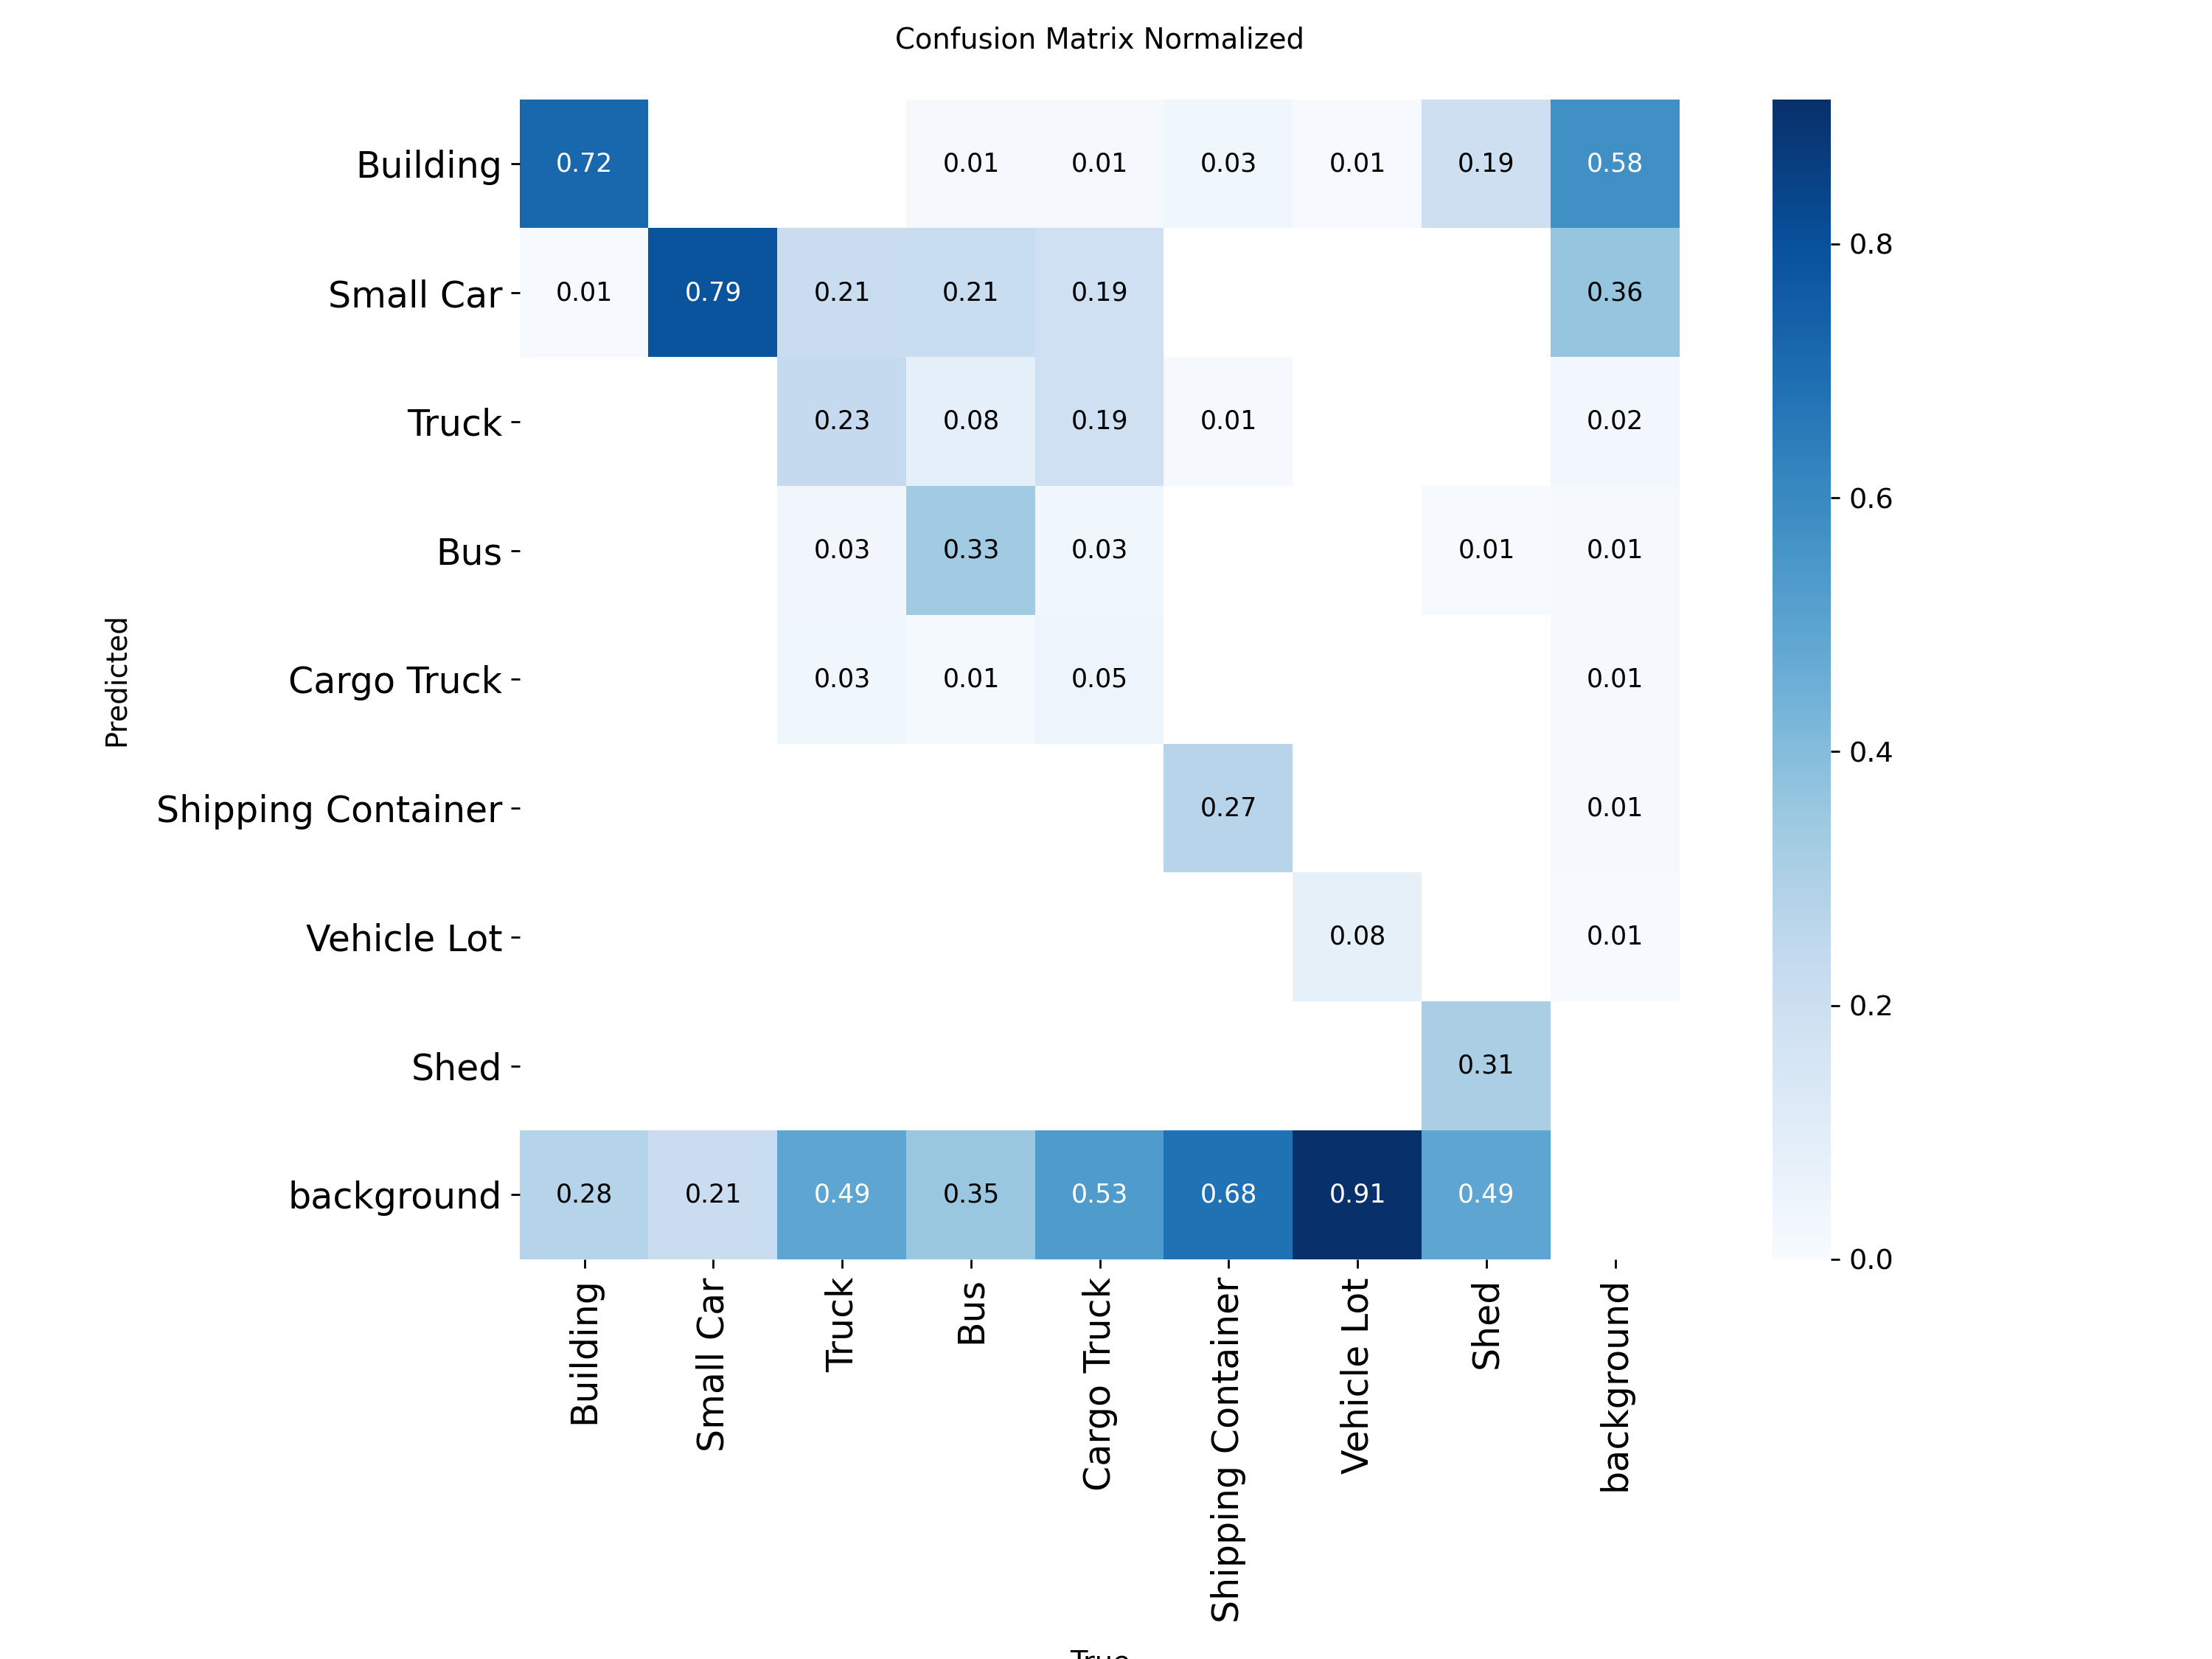
\includegraphics[width=0.75\linewidth]{results/confusion_matrices/acsyolo_on_CZB/confusion_matrix_normalized.png}
\caption{Normalized confusion matrix of the ACS-YOLO model evaluated on the CZ\_B (temperate zone) OOD test set. Small objects (Shed, Cargo Truck) and Vehicle Lot suffer from high background confusion (FN rate of 49\%, 53\%, and 91\% respectively), while Shipping Containers show moderate confusion with Buildings (3\%).}
\label{fig:confusion_matrix}
\end{figure}

Failure cases predominantly occur in three scenarios. First, small objects such as Cargo Truck and Shed are frequently missed across all methods because their pixel footprint at $640\times640$ resolution is often below the detection threshold. Second, the Vehicle Lot class suffers from high intra-class variability---parking areas in temperate zones appear visually distinct from those in arid regions, making cross-domain recognition inherently difficult. Third, Shipping Container detections are occasionally confused with Building edges or rooftop segments, particularly in high-density urban areas within CZ\_B.


% =====================================================================
\section{Additional Study}
% =====================================================================

\subsection{Per-Class Cross-Domain Analysis}

Table~\ref{tab:perclass} presents the per-class mAP@50-95 breakdown for the DG-Aug method across all three OOD configurations, illustrating which object categories benefit most from domain-generalisation augmentation.

\begin{table}[H]
\centering
\caption{Per-class mAP@50-95 for DG-Aug across OOD configurations. Asterisk (*) denotes OOD zone.}
\label{tab:perclass}
\small
\begin{tabular}{lcccccccc}
\toprule
\textbf{Zone} & \textbf{Building} & \textbf{Sm.\ Car} & \textbf{Truck} & \textbf{Bus} & \textbf{Cargo T.} & \textbf{Ship.\ C.} & \textbf{Veh.\ Lot} & \textbf{Shed} \\
\midrule
\multicolumn{9}{l}{\textit{OOD target = CZ\_A}} \\
CZ\_A* & 26.22 & 23.58 & 14.75 & 12.76 & 2.74 & 11.43 & 2.11 & 6.07 \\
CZ\_B  & 38.73 & 29.44 & 13.52 & 19.56 & 6.80 & 7.00 & 2.38 & 13.96 \\
CZ\_C  & 32.68 & 23.60 &  8.82 &  8.07 & 6.49 & 1.20 & 1.95 &  3.14 \\
\midrule
\multicolumn{9}{l}{\textit{OOD target = CZ\_B}} \\
CZ\_A  & 31.77 & 25.87 & 17.19 & 12.08 & 2.84 & 12.16 & 3.14 & 9.04 \\
CZ\_B* & 34.18 & 22.97 &  9.19 & 11.66 & 4.91 & 6.06 & 1.82 & 6.24 \\
CZ\_C  & 32.45 & 22.15 &  6.43 &  7.13 & 6.42 & 0.86 & 3.16 & 4.18 \\
\midrule
\multicolumn{9}{l}{\textit{OOD target = CZ\_C}} \\
CZ\_A  & 31.40 & 25.29 & 17.71 & 10.24 & 3.16 & 13.44 & 2.58 & 8.68 \\
CZ\_B  & 38.03 & 27.57 & 12.98 & 18.32 & 5.73 & 5.63 & 2.80 & 10.44 \\
CZ\_C* & 28.78 & 19.21 &  6.94 &  7.28 & 6.44 & 2.85 & 3.36 & 2.64 \\
\bottomrule
\end{tabular}
\end{table}

Building and Small Car consistently achieve the highest mAP@50-95 across all zones, exceeding 19\% even in OOD settings. These classes benefit from large sample sizes and relatively stable visual appearance across climate zones. In contrast, Vehicle Lot, Shed, and Cargo Truck remain below 7\% in most OOD configurations, suggesting that their cross-domain appearance variability exceeds what current augmentation strategies can bridge.

\begin{figure}[H]
\centering
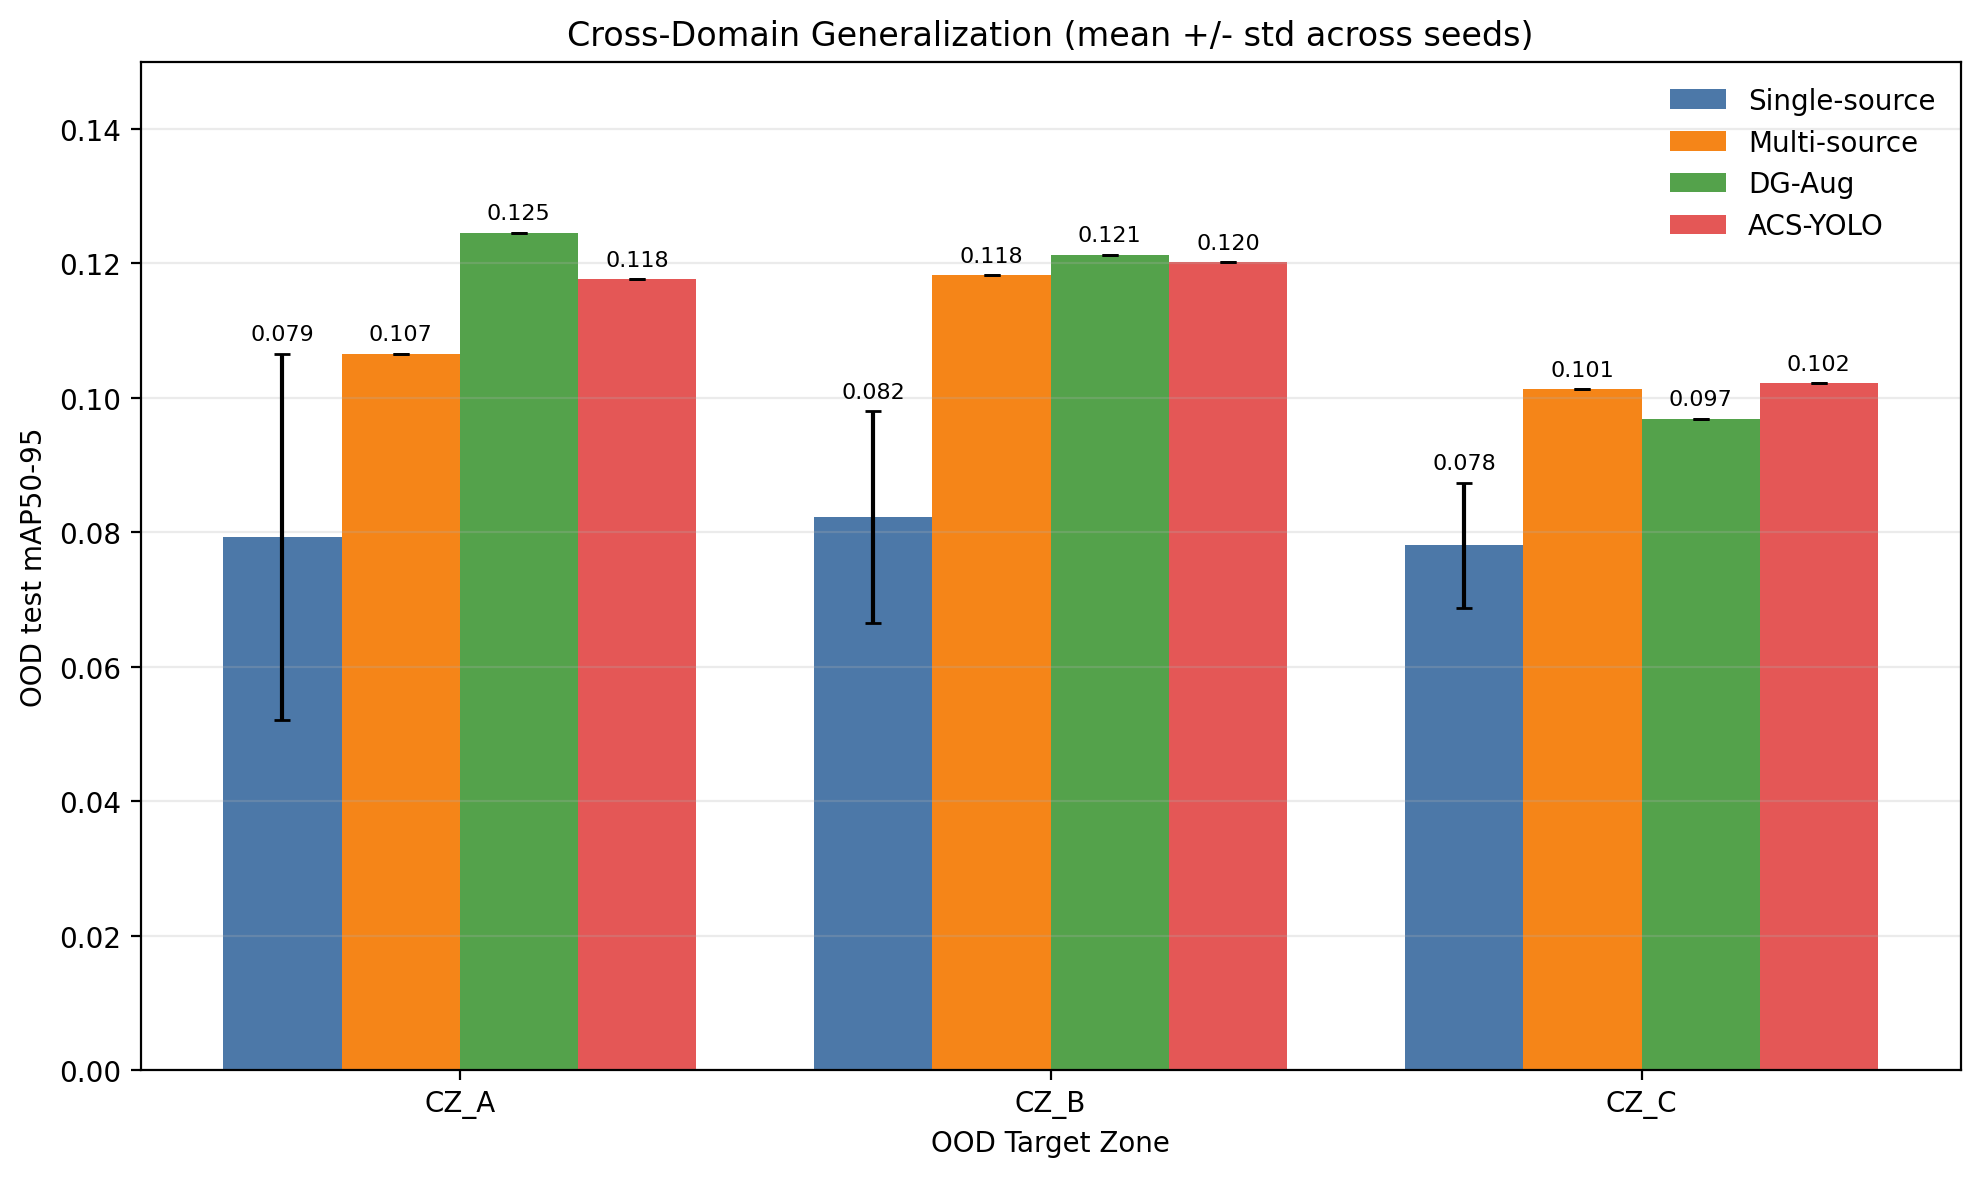
\includegraphics[width=0.48\linewidth]{results/official/plots/ood_map_by_zone.png}
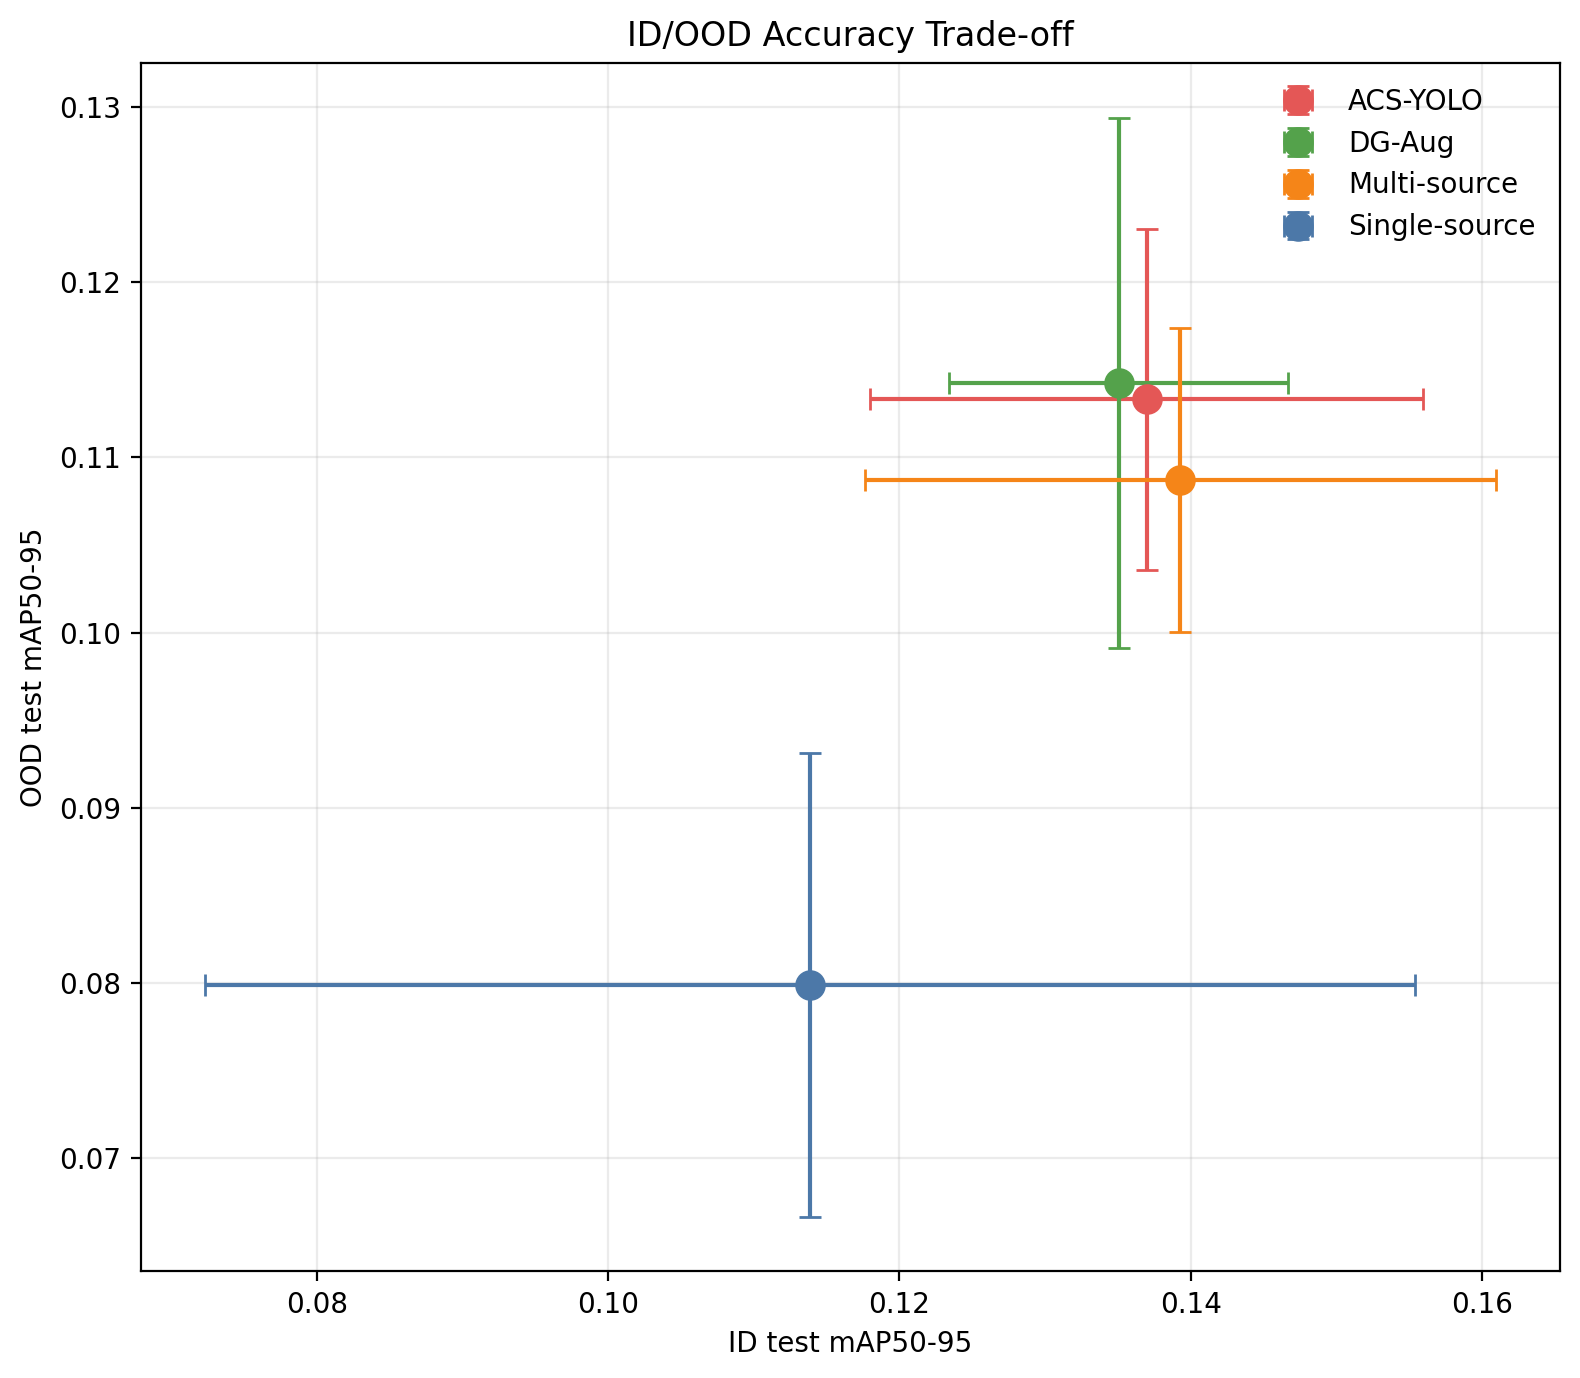
\includegraphics[width=0.48\linewidth]{results/official/plots/id_ood_tradeoff.png}
\caption{Left: OOD mAP@50-95 by zone and method. Right: ID--OOD trade-off scatter plot showing that DG-Aug and ACS-YOLO achieve better OOD performance without significantly sacrificing ID accuracy.}
\label{fig:official_plots}
\end{figure}


% =====================================================================
\section{Discussion}
% =====================================================================

The experimental results confirm that distribution shifts across climate zones cause meaningful performance degradation in satellite object detection, consistent with the findings of Al-Emadi et al.~\cite{alemadi2025rwds}. Even the simple strategy of multi-source training---pooling data from two climate zones---reduces average PD from 20.95\% to 15.69\% at mAP@50, demonstrating that exposure to greater visual diversity during training is beneficial. DG-Aug further reduces PD to 11.01\% by introducing climate-aware augmentations that simulate atmospheric, colour, and texture variations characteristic of different geographic regions. This finding suggests that a substantial portion of the domain gap in satellite imagery can be attributed to low-level visual differences (colour palette, contrast, haze) rather than high-level semantic shifts.

ACS-YOLO achieves comparable results to DG-Aug (average PD of 11.81\%) through a fundamentally different mechanism: rather than augmenting the data, it identifies and down-weights training samples that exhibit domain-specific artefacts that do not generalise across zones. This complementary approach is particularly effective for the CZ\_C target direction, where ACS-YOLO achieves the highest H-score (29.50\%) among all methods. The adaptive weighting mechanism may be mitigating the impact of zone-specific visual patterns (e.g., distinctive tropical vegetation textures) that confuse the detector when encountered in other domains.

Several limitations should be acknowledged. First, all experiments use a single random seed (42), which limits the statistical power of the comparisons. Future work should employ multiple seeds and report confidence intervals. Second, the YOLOv8n architecture is the only backbone evaluated; the effectiveness of DG-Aug and ACS-YOLO on Transformer-based detectors (e.g., DINO, Grounding DINO) remains an open question. Third, the current augmentation strategy in DG-Aug is manually designed based on domain knowledge about climate-zone characteristics; learning the augmentation policy automatically could yield further improvements. Finally, the relatively low absolute mAP values (below 30\% even in ID settings) suggest that satellite object detection on the xView dataset is inherently challenging, and future research should explore more powerful backbone architectures and larger training datasets.


% =====================================================================
\section{Conclusion}
% =====================================================================

This report presented a systematic empirical study of object detection robustness under real-world distribution shifts in satellite imagery. Using the RWDS climate-zone benchmark with the YOLOv8n detector, four training strategies were compared: single-source baseline, multi-source baseline, DG-Aug, and ACS-YOLO. The key findings are as follows. Multi-source training reduces average performance degradation from 20.95\% to 15.69\% at mAP@50 by leveraging visual diversity from multiple climate zones. DG-Aug achieves the lowest average PD of 11.01\% through targeted augmentations that simulate cross-climate visual variations, and attains the best harmonic mean of 30.03\% when CZ\_A is the OOD target. ACS-YOLO provides a complementary approach based on adaptive sample weighting, achieving competitive performance with average PD of 11.81\%. Per-class analysis reveals that large, visually stable classes (Building, Small Car) benefit most from generalisation strategies, while small, rare objects (Vehicle Lot, Shed) remain challenging across all methods.

Future work should explore automatic augmentation policy learning, Transformer-based detection backbones, multi-seed evaluation for statistical robustness, and extension to the RWDS disaster-response benchmark datasets.


% =====================================================================
\section*{References}
\addcontentsline{toc}{section}{References}
% =====================================================================

\begin{thebibliography}{99}

\bibitem{alemadi2025rwds}
S.~Al-Emadi, Y.~Yang, and F.~Ofli, ``Benchmarking object detectors under real-world distribution shifts in satellite imagery,'' in \textit{Proceedings of the IEEE/CVF Conference on Computer Vision and Pattern Recognition (CVPR)}, 2025. arXiv:2503.19202.

\bibitem{shermeyer2020xview}
J.~Shermeyer and A.~Van Etten, ``The effects of super-resolution on object detection performance in satellite imagery,'' in \textit{Proceedings of the IEEE/CVF Conference on Computer Vision and Pattern Recognition Workshops}, 2019, pp.~0--0.

\bibitem{beck2018koppen}
H.~E.~Beck, N.~E.~Zimmermann, T.~R.~McVicar, N.~Vergopolan, A.~Berg, and E.~F.~Wood, ``Present and future K\"{o}ppen-Geiger climate classification maps at 1-km resolution,'' \textit{Scientific Data}, vol.~5, no.~1, pp.~1--12, 2018.

\bibitem{jocher2023yolov8}
G.~Jocher, A.~Chaurasia, and J.~Qiu, ``Ultralytics YOLO,'' 2023. [Online]. Available: \url{https://github.com/ultralytics/ultralytics}

\bibitem{redmon2016yolo}
J.~Redmon, S.~Divvala, R.~Girshick, and A.~Farhadi, ``You only look once: Unified, real-time object detection,'' in \textit{Proceedings of the IEEE Conference on Computer Vision and Pattern Recognition}, 2016, pp.~779--788.

\bibitem{ren2015fasterrcnn}
S.~Ren, K.~He, R.~Girshick, and J.~Sun, ``Faster R-CNN: Towards real-time object detection with region proposal networks,'' in \textit{Advances in Neural Information Processing Systems}, vol.~28, 2015.

\bibitem{carion2020detr}
N.~Carion, F.~Massa, G.~Synnaeve, N.~Usunier, A.~Kirillov, and S.~Zagoruyko, ``End-to-end object detection with Transformers,'' in \textit{European Conference on Computer Vision}, 2020, pp.~213--229.

\bibitem{zhang2022dino}
H.~Zhang, F.~Li, S.~Liu, L.~Zhang, H.~Su, J.~Zhu, L.~M.~Ni, and H.-Y.~Shum, ``DINO: DETR with improved denoising anchor boxes for end-to-end object detection,'' in \textit{International Conference on Learning Representations}, 2023.

\bibitem{wang2022domainsurvey}
J.~Wang, C.~Lan, C.~Liu, Y.~Ouyang, T.~Qin, W.~Lu, Y.~Chen, W.~Zeng, and P.~Yu, ``Generalizing to unseen domains: A survey on domain generalization,'' \textit{IEEE Transactions on Knowledge and Data Engineering}, vol.~35, no.~8, pp.~8052--8072, 2022.

\bibitem{zhou2022dg}
K.~Zhou, Z.~Liu, Y.~Qiao, T.~Xiang, and C.~C.~Loy, ``Domain generalization: A survey,'' \textit{IEEE Transactions on Pattern Analysis and Machine Intelligence}, vol.~45, no.~4, pp.~4396--4415, 2022.

\bibitem{volpi2018adversarial}
R.~Volpi, H.~Namkoong, O.~Sener, J.~C.~Duchi, V.~Murino, and S.~Savarese, ``Generalizing to unseen domains via adversarial data augmentation,'' in \textit{Advances in Neural Information Processing Systems}, vol.~31, 2018.

\bibitem{xu2020adversarialaugment}
M.~Xu, J.~Zhang, B.~Ni, T.~Li, C.~Wang, Q.~Tian, and W.~Zhang, ``Adversarial domain adaptation with domain mixup,'' in \textit{AAAI Conference on Artificial Intelligence}, 2020, pp.~6502--6509.

\bibitem{li2018domaincondbn}
Y.~Li, N.~Wang, J.~Shi, J.~Liu, and X.~Hou, ``Revisiting batch normalization for practical domain adaptation,'' in \textit{International Conference on Learning Representations Workshop}, 2018.

\bibitem{pan2018batchinstance}
S.~H.~Pan, Q.~Yang, ``A survey on transfer learning,'' \textit{IEEE Transactions on Knowledge and Data Engineering}, vol.~22, no.~10, pp.~1345--1359, 2010.

\bibitem{buslaev2020albumentations}
A.~Buslaev, V.~I.~Iglovikov, E.~Khvedchenya, A.~Parinov, M.~Druzhinin, and A.~A.~Kalinin, ``Albumentations: Fast and flexible image augmentations,'' \textit{Information}, vol.~11, no.~2, p.~125, 2020.

\bibitem{zhang2023adacs}
X.~Zhang, J.~C.~Stendahl, L.~H.~Staib, A.~J.~Sinusas, A.~Wong, and J.~S.~Duncan, ``Adaptive correspondence scoring for unsupervised medical image registration,'' \textit{arXiv preprint arXiv:2312.00837}, 2023.

\end{thebibliography}

\end{document}
